\documentclass[11pt]{article}

\usepackage[margin=1in]{geometry}
\usepackage[T1]{fontenc}
\usepackage{lmodern}
\usepackage{amsmath,amssymb,mathtools}
\usepackage{enumitem}
\usepackage{microtype}
\usepackage{xcolor}
\usepackage{titlesec}
\usepackage{fancyhdr}
\usepackage{booktabs}
\usepackage{graphicx}
\usepackage{listings}
\usepackage{needspace}

\definecolor{accent}{HTML}{9A3412}
\definecolor{softgray}{HTML}{F7F7F4}
\definecolor{textgray}{HTML}{3F3F46}
\definecolor{codegreen}{HTML}{166534}
\definecolor{codeblue}{HTML}{1D4ED8}
\definecolor{codepurple}{HTML}{7C3AED}
\definecolor{codeborder}{HTML}{D6D3D1}

\lstdefinestyle{pythoncode}{
  language=Python,
  basicstyle=\small\ttfamily,
  keywordstyle=\color{codeblue}\bfseries,
  stringstyle=\color{codegreen},
  commentstyle=\color{textgray}\itshape,
  identifierstyle=\color{black},
  emph={jax,jnp,functools,mesh},
  emphstyle=\color{codepurple},
  backgroundcolor=\color{softgray},
  frame=single,
  rulecolor=\color{codeborder},
  framerule=0.4pt,
  framesep=6pt,
  xleftmargin=0.5em,
  xrightmargin=0.5em,
  aboveskip=0.5em,
  belowskip=0.7em,
  columns=fullflexible,
  keepspaces=true,
  showstringspaces=false,
  breaklines=true,
  breakatwhitespace=false,
  tabsize=2
}

\pagestyle{fancy}
\fancyhf{}
\lhead{\textcolor{textgray}{Scaling Book Exercises}}
\rhead{\textcolor{textgray}{\thepage}}
\renewcommand{\headrulewidth}{0.3pt}

\titleformat{\section}
  {\Large\bfseries\color{accent}}
  {Part \thesection}{0.75em}{}
\titleformat{\subsection}
  {\large\bfseries\color{textgray}}
  {Exercise \thesubsection}{0.75em}{}
\titleformat{\paragraph}
  {\normalsize\bfseries\color{textgray}}
  {}{0pt}{}

\titlespacing*{\section}{0pt}{1.8em}{1.0em}
\titlespacing*{\subsection}{0pt}{1.5em}{0.45em}
\titlespacing*{\paragraph}{0pt}{1.2em}{0.45em}

\setlist[enumerate]{leftmargin=*, itemsep=0.65em, topsep=0.45em}
\setlength{\parindent}{0pt}
\setlength{\parskip}{0.55em}
\setlength{\headheight}{14pt}
\setlength{\abovedisplayskip}{0.45em}
\setlength{\belowdisplayskip}{0.45em}
\setlength{\abovedisplayshortskip}{0.35em}
\setlength{\belowdisplayshortskip}{0.35em}
\renewcommand{\arraystretch}{1.2}

\newcommand{\B}{B}
\newcommand{\D}{D}
\newcommand{\F}{F}
\newcommand{\W}{W}
\newcommand{\lam}{\lambda}
\newcommand{\flops}{\mathrm{FLOP/s}}
\newcommand{\bytes}{\mathrm{bytes}}
\newcommand{\bfloat}{\mathrm{bf16}}
\newcommand{\us}{\mu\mathrm{s}}
\newcommand{\ms}{\mathrm{ms}}
\newcommand{\exercisebreak}{\Needspace{8\baselineskip}}
\newcommand{\quizbreak}{\Needspace{6\baselineskip}}

\title{\Huge \textbf{Scaling Book Exercises}}
\author{}
\date{}

\begin{document}
\maketitle
\thispagestyle{empty}

\section{}

\exercisebreak
\subsection{}
\begin{enumerate}
  \item Load $\B\D + \D\F$ and write back $\B\F$.

  \item Each output element requires $\D$ multiplications and $\D$ additions, so the total work is
  \[
    2\D\B\F .
  \]

  \item Per formula, the arithmetic intensity is
  \[
    \frac{2\D\B\F}{\B\D+\D\F+\B\F}.
  \]

  \item Per formula,
  \[
    T_{\mathrm{math}}=\frac{2\B\D\F}{3.94\times 10^{14}},
    \qquad
    T_{\mathrm{comm}}=\frac{\B\D+\D\F+\B\F}{8.2\times 10^{11}}.
  \]
  The lower bound is $\max(T_{\mathrm{math}},T_{\mathrm{comm}})$ and the upper bound is $T_{\mathrm{math}}+T_{\mathrm{comm}}$.
\end{enumerate}

\exercisebreak
\subsection{}
We still have $2\B\D\F$ bfloat16 operations. Assuming $\B$ is relatively small, we load $\D\F$ bytes, thus the intensity is $2\B$ and the accelerator intensity is $240$. For compute-bound execution,
\[
  2\B > 240 \quad\Longrightarrow\quad \B > 120.
\]

\exercisebreak
\subsection{}
\begin{center}
  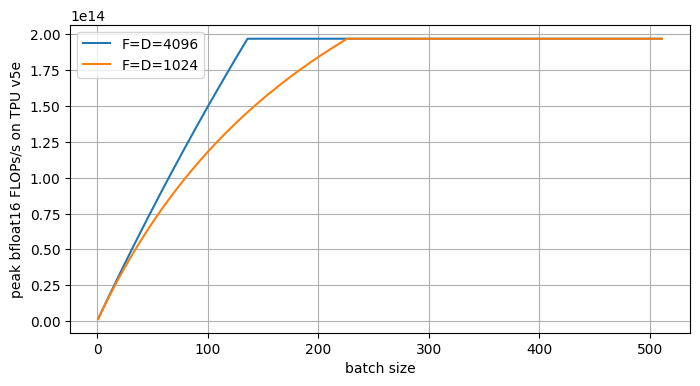
\includegraphics[width=0.82\linewidth]{fig/1-3.png}
\end{center}

\exercisebreak
\subsection{}
We have the same $2\B\D\F$ FLOPs, but the load is now
\[
  \B\D+\B\D\F+\B\F.
\]
Because $\B\D\F$ dominates, the intensity is roughly constant:
\[
  \mathrm{intensity} \approx 2.
\]

\exercisebreak
\subsection{}
We have $1.97\times 10^{15}$ bfloat16 FLOPs with sparsity, and half of that without sparsity:
\[
  9.89\times 10^{14}.
\]
The bandwidth is $3.35\times 10^{12}$, so the compute-bound batch threshold is
\[
  \frac{9.89\times 10^{14}}{3.35\times 10^{12}}
  \approx 295.
\]

\section{}

\exercisebreak
\subsection{}
We have $2.2\times 10^{11}=4\times 10^{11}$ total bytes, so this is $1.25\times 10^{10}$ bytes per chip. The bandwidth of each chip is $1.23\times 10^{12}$ bytes/s, so the full load takes about
\[
  10\ \ms.
\]

\exercisebreak
\subsection{}
For a v5e pod, the pod has $16\times 16$ chips and 8 chips per host, so there are 32 total hosts and 256 tensor cores. Total FLOPs/s is
\[
  256\cdot 1.97\times 10^{14}=5.04\times 10^{16}.
\]
Each chip has $16$ GB of HBM, so the total is
\[
  256\cdot 16 = 4\ \mathrm{TB}.
\]

For a v5p pod, the pod has $16\times 20\times 28$ chips and 4 chips per host, so there are 2240 hosts and 2 cores per chip. Total FLOPs/s is
\[
  8960\cdot 4.59\times 10^{14}\approx 4.1\times 10^{18}.
\]
Each chip has 96 GB of HBM, so the total is
\[
  8960\cdot 96 = 860\ \mathrm{TB}.
\]

\exercisebreak
\subsection{}
For compute, we have $2\B\D\F$ operations, which takes time
\[
  \frac{2\B\D\F}{9.2\times 10^{14}}.
\]
The load/store is
\[
  2(\B\D+\D\F+\B\F),
\]
and with PCIe this takes
\[
  \frac{2(\B\D+\D\F+\B\F)}{1.6\times 10^{10}}.
\]

For compute-bound execution, with assumptions:
\[
  \frac{8\B\D^2}{9.2\times 10^{14}}
  >
  \frac{8\D^2}{1.6\times 10^{10}}
  \quad\Longrightarrow\quad
  \B > 57500.
\]

\exercisebreak
\subsection{}
\begin{enumerate}
  \item FLOPs are
  \[
    2\cdot 4096\cdot 16384\cdot \B.
  \]
  Load/write is
  \[
    16384\cdot 4096 + 4096\B + 16384\B.
  \]
  With full overlap, the total time is
  \[
    \max\left\{
      \frac{1.3\times 10^8\B}{3.94\times 10^{14}},
      \frac{6.7\times 10^7+2\times 10^4\B}{8.2\times 10^{11}}
    \right\}.
  \]

  \item The only change is the $T_{\mathrm{comm}}$ denominator. VMEM bandwidth is about $22\times$ higher, so total time is
  \[
    \max\left\{
      \frac{1.3\times 10^8\B}{3.94\times 10^{14}},
      \frac{6.7\times 10^7+2\times 10^4\B}{8.2\times 10^{11}\cdot 22}
    \right\}.
  \]
\end{enumerate}

\exercisebreak
\subsection{}
\begin{enumerate}
  \item We first see that we have 6 hops because there is no wrap connection. Thus, the first byte will arrive in $6\us$.

  \item We have total data
  \[
    2\cdot 8\cdot 128\cdot 8192\approx 1.7\times 10^7\ \bytes.
  \]
  We also have 2 outputs and 2 inputs, so total bandwidth is
  \[
    2\cdot 4.5\times 10^{10}=9\times 10^{10}.
  \]
  Thus the total time is
  \[
    \frac{1.7\times 10^7}{9\times 10^{10}}\approx 188\us.
  \]

  \item It is likely faster to load each chunk to the correct TPU, then use ICI because of the higher bandwidth. Total data is
  \[
    128\cdot 1024\cdot 128\cdot 1024 = 16\ \mathrm{GB}.
  \]
  For the PCIe load, this is $1$ GB with bandwidth $1.6\times 10^{10}$, which takes about $63\ms$.

  For ICI copy, the lower bound is that $15$ GB is received by TPU $\{0,3\}$ with total bandwidth $9\times 10^{10}$, so the bound is $167\ms$.

  We then copy $16$ GB plus a small $2$ MB vector from HBM to MXU, which takes only about $20\ms$.

  Within MXU, we have
  \[
    2\cdot 8\cdot 128\cdot 1024\cdot 128\cdot 1024
  \]
  FLOPs with $1.97\times 10^{14}$ FLOPs/s, which gives less than $2\ms$.

  Thus the upper bound is the sum of these times, and the lower bound is the maximum, $167\ms$.
\end{enumerate}

\quizbreak
\paragraph{Pop Quiz}
We have $4\cdot 8\cdot 128$ ALUs, which can each do 1 FLOP/cycle, so the total is
\[
  4096\ \mathrm{FLOPs/cycle}.
\]
At clock speed $1.75$ GHz, this gives
\[
  1.75\times 10^9\ \mathrm{cycles/s},
  \qquad
  \text{so total } 7\times 10^{12}\ \flops.
\]

\section{}

\quizbreak
\paragraph{Pop Quiz}
Each shard is of size
\[
  \left[\frac{1024}{16},4096\right]=[64,4096].
\]
So each GPU has
\[
  4\cdot 64\cdot 4096 = 1\ \mathrm{MB},
\]
and the load time is
\[
  \frac{10^6}{3.4\times 10^{12}}\approx 294\ \mathrm{ns}.
\]

\quizbreak
\paragraph{Pop Quiz}
Each shard is of size
\[
  \left[\frac{128}{16},2048\right]=[8,2048].
\]
So each device has
\[
  8\cdot 2048 = 16\ \mathrm{KB},
\]
and total memory is
\[
  16\cdot 32 = 512\ \mathrm{KB}.
\]

\quizbreak
\paragraph{Pop Quiz}
Each shard is
\[
  512\cdot 8192\cdot 2 = 8\ \mathrm{MB},
\]
and the total array has size $32$ MB. We do not have wrap-around, so we have to do 3 unidirectional hops:
\[
  \frac{3\cdot 8\times 10^6}{4.5\times 10^{10}}
  \approx 533\us.
\]
In part 2, each shard is only
\[
  64\cdot 256\cdot 2=32\ \mathrm{KB},
\]
so each hop is
\[
  \frac{32\times 10^3}{4.5\times 10^{10}}\approx 0.7\us.
\]
We know the minimum latency is $1\us$, so the total will be $3\us$.

\exercisebreak
\subsection{}
Say that $A$ has size $S$. Each shard has size $S/4$ and is stored on 16 devices, so the total bytes are $4S$. Thus, the ratio is $4$.

\exercisebreak
\subsection{}
We have
\[
  V=\frac{2\B\D}{Y}
  =
  \frac{2\cdot 1024\cdot 4096}{4}
  =
  2\ \mathrm{MB}.
\]
Because the $Y$-axis stays sharded, we have wraparound, so bidirectional communication gives
\[
  \frac{2\times 10^6}{9\times 10^{10}}\approx 22\us.
\]

For $\mathrm{AllGather}_{xy}$, we double the bandwidth but $V$ is $4\times$ larger, so the time is $2\times$ larger, about $44\us$.

For $\mathrm{AllReduce}$, we have size
\[
  \frac{2\B\D}{XY}
  =
  \frac{1024\cdot 4096}{8}
  =
  512\ \mathrm{KB}.
\]
The cost is $2\times$ that of all-gather, and the bidirectional time is
\[
  \frac{512\times 10^3\cdot 2}{9\times 10^{10}}\approx 11\us.
\]

\exercisebreak
\subsection{}
This is a total array of $256$ bytes, or $64$ per shard, so latency is certainly the bound. We have wraparound, so bidirectional communication means at most 2 hops, hence $2\us$.

\exercisebreak
\subsection{}
For the baseline, all-gather has time
\[
  \frac{2\D\F}{\W}.
\]
We have $2\B\D\F$ FLOPs and compute time
\[
  \frac{2\B\D\F}{\lam}.
\]
Assuming overlap, total time is
\[
  \max\left\{\frac{2\D\F}{\W},\frac{2\B\D\F}{\lam}\right\}.
\]

For the new strategy, each shard does
\[
  \frac{2\B\D\F}{X}
\]
FLOPs in time
\[
  \frac{2\B\D\F}{X\lam}.
\]
For the all-reduce, bytes are $2\B\F$, so the time is
\[
  \frac{4\B\F}{\W}.
\]
Therefore the total is
\[
  \max\left\{\frac{4\B\F}{\W},\frac{2\B\D\F}{X\lam}\right\}.
\]

For strategy 1, communication bound when
\[
  \B < \frac{\lam}{\W}.
\]
This ratio is roughly $2000$ for v5e.

For strategy 2, communication bound when
\[
  X < \frac{\D}{4000}.
\]
With $\D$ on the order of less than $10000$, this is probably true, so it is communication bound.

When $\B<2000$, strategy 2 is better if
\[
  \frac{4\B\F}{\W}<\frac{2\D\F}{\W}
  \quad\Longrightarrow\quad
  \D>2\B,
\]
which is often true for these small batches.

When $\B>2000$, strategy 2 is better if
\[
  \frac{4\B\F}{\W}<\frac{2\B\D\F}{\lam}
  \quad\Longrightarrow\quad
  \D>4000,
\]
which is true for large models.

\exercisebreak
\subsection{}
Let us go through a few options.

\begin{enumerate}[label=(\alph*)]
  \item Shard $I$ across $XYZ$:
  \[
    \frac{\mathrm{FLOPs}}{\mathrm{TPU}}=\frac{2IJK}{64},
    \qquad
    T_{\mathrm{compute}}=\frac{IJK}{32\lam}.
  \]
  Then we do all-gather with $V=2IK$, so
  \[
    T_{\mathrm{comm}}=\frac{2IK}{3\W}.
  \]

  \item Shard $K$ across $XYZ$: this will trivially be the same as above.

  \item Shard $J$ across $XYZ$: FLOPs/TPU are the same, so compute time is the same. Now we have to do all-reduce, which has double cost:
  \[
    T_{\mathrm{comm}}=\frac{4IK}{3\W}.
  \]

  \item Full replicate:
  \[
    \frac{\mathrm{FLOPs}}{\mathrm{TPU}}=2IJK,
    \qquad
    T_{\mathrm{compute}}=\frac{2IJK}{\lam},
  \]
  and there is no communication time.
\end{enumerate}

Thus, option (c) is clearly worse; options (a) and (b) are equally good. Option (d) is probably worse most times because the compute cost is $64\times$ worse.

\exercisebreak
\subsection{}
We have $\W$ as bidirectional ICI bandwidth and $\lam$ as bfloat16 FLOPs/s.

\begin{enumerate}[label=(\alph*)]
  \item We first do sharded matmul, which has FLOPs
  \[
    \frac{2IJK}{4\cdot 4}
  \]
  and compute time
  \[
    \frac{IJK}{8\lam}.
  \]
  We then do all-reduce with
  \[
    V=\frac{2IK}{4}.
  \]
  But we have no wrap-around, so we have 3 hops and $\W/2$ for unidirectional bandwidth. Therefore all-reduce will take
  \[
    2\cdot 3\cdot \frac{V/4}{\W/2}
    =
    \frac{3IK}{2\W}.
  \]
  Thus
  \[
    T_{\mathrm{compute}}=\frac{IJK}{8\lam},
    \qquad
    T_{\mathrm{comm}}\approx \frac{3IK}{2\W}.
  \]

  \item Here we will first all-gather
  \[
    B[J_x,K_y]\to B[J,K_y].
  \]
  The $V$ here is $2JK/16$, and again we have 3 hops with $\W/2$ bandwidth, so
  \[
    T_{\mathrm{comm}}=\frac{3JK}{4\W}.
  \]
  Now we have $2IJK/16$ FLOPs, so
  \[
    T_{\mathrm{compute}}=\frac{IJK}{8\lam}.
  \]

  \item Here we do not have to do any communication, and each chip has FLOPs
  \[
    \frac{2IJK}{4\cdot 4},
  \]
  so
  \[
    T_{\mathrm{compute}}=\frac{IJK}{8\lam}.
  \]
\end{enumerate}

\exercisebreak
\subsection{}
The matrices have size
\[
  2\cdot 8192\cdot 32768\approx 512\ \mathrm{MB},
\]
so they must be sharded. We also want to avoid all-gathering the weights, and we should likely shard the input along $\D$, so
\[
  \mathrm{In}[B,D_{xy}].
\]
Now, we can shard $\W$ along $\D$ or $\F$, but if we do $\D$ then we have to reduce into $B\times F$, which is larger than $B\times D$. Thus it seems best to do
\[
  \mathrm{In}[B,D_{xy}]
  \cdot
  W_{\mathrm{in}}[D,F_{xy}]
  \cdot
  W_{\mathrm{out}}[F_{xy},D]
  \to
  \mathrm{Out}[B,D_{xy}].
\]

First, we all-gather $\mathrm{In}$ on $XY$, so
\[
  V=2\B\D=2\cdot 128\cdot 8192=2\ \mathrm{MB}.
\]
We have 2 axes, so
\[
  T_{\mathrm{AG}}=\frac{2\times 10^6}{2.9\times 10^{10}}\approx 11\us.
\]

We then shard multiply:
\[
  \mathrm{In}[B,D]\cdot W_{\mathrm{in}}[D,F_{xy}]
  \to H[B,F_{xy}].
\]
Each chip has
\[
  \frac{2\B\D\F}{4}\approx 17\times 10^9
\]
FLOPs, and the compute time is
\[
  \frac{17\times 10^9}{1.97\times 10^{14}}\approx 86\us.
\]

The next matmul is
\[
  H[B,F_{xy}]\cdot W_{\mathrm{out}}[F_{xy},D]\to \mathrm{Out}[B,D],
\]
which has the same FLOPs and time.

Finally, we just do reduce-scatter over $X,Y$ with
\[
  V=2\B\D\approx 2\ \mathrm{MB},
  \qquad
  T_{\mathrm{RS}}\approx \frac{2\times 10^6}{2.9\times 10^{10}}\approx 11\us.
\]
Thus, about $22\us$ communication and $172\us$ on FLOPs.

\exercisebreak
\subsection{}
\[
\begin{array}{@{}lr@{}}
\toprule
\text{collective} & \text{time} \\
\midrule
\text{AllGather} & 0.705\ \ms \\
\text{ReduceScatter} & 0.980\ \ms \\
\text{AllReduce} & 0.977\ \ms \\
\text{AllToAll} & 0.409\ \ms \\
\bottomrule
\end{array}
\]

We see AllToAll being the cheapest as expected, but we see that AllReduce is not $2\times$ the time of AllGather and ReduceScatter as we may expect, potentially due to some XLA optimizations.

\exercisebreak
\subsection{}
\begin{enumerate}
  \item This is simple. We just do a traditional matmul, treating the second matrix as sharded, to build $T[N,K]$, where
  \[
    t_{nk}=\sum_j a_{nj}b_{jk},
  \]
  and $j$ is limited to only the relevant shard indices. Finally, we just do all-reduce over $T[N,K]\{u_x\}$ to get the final $T[N,K]$.

  \item We just do not do all-reduce. Instead, cheaper reduce-scatter to something like
  \[
    T[N,K]\{u_x\}\to T[N_x,K].
  \]
\end{enumerate}

\exercisebreak
\subsection{}
\begin{enumerate}
  \item Each ``shard'' has
  \[
    \frac{N}{D}\cdot N = \frac{N^3}{D}
  \]
  elements, and in the single-direction case there are $D-1$ hops, so transfer is
  \[
    \frac{N^3(D-1)}{D}
  \]
  scalars.

  \item We have cascading transfer, so chunks move $D-1,D-2,\ldots,1$ times, which is
  \[
    \frac{D(D-1)}{2}.
  \]
  Each of these smaller chunks is
  \[
    \frac{N}{D}\cdot \frac{N}{D}=\frac{N^2}{D^2}.
  \]
  So total scalars are
  \[
    \frac{D(D-1)N^2}{2D^2}
    =
    \frac{N^2(D-1)}{2D}.
  \]

  \item The ratio is $1/2$, so all-to-all is half the cost because we have the reducing sum
  \[
    D-1+D-2+\cdots+1
  \]
  instead of
  \[
    D-1+D-1+\cdots+D-1.
  \]

  \item We simply halve the number of scalars because we push half the data in the opposite direction.

  \item Our cascading sum becomes
  \[
    \frac{D}{2}+\frac{D}{2}-1+\cdots+1
    =
    \frac{D/2(D/2+1)}{2}
    \to
    \frac{D^2}{8}.
  \]
  In the single-direction limit this was $D^2/2$, so we improve by a factor of $4$.

  \item We had $2\times$ speed for single direction. In bidirectional mode, all-gather has a $2\times$ improvement and all-to-all has a $4\times$ improvement, so we have another net $2\times$ gain, giving $4\times$ total gain.
\end{enumerate}

\clearpage
\section{}

\exercisebreak
\subsection{}
We have per-layer
\[
  3\D\F + 4\D N H + \D.
\]
We also have $\D V$ for vocab and $\D V$ for unembed, so total is
\[
  L(3\D\F + 4\D N H + \D) + 2\D V \approx 16\mathrm{B}
\]
parameters total.

Attention per layer has
\[
  4\D N H = 4\D^2,
\]
and MLPs have
\[
  3\D\F = 12\D^2.
\]
Ignoring the second-order terms, the fraction is
\[
  \frac{4}{16}\approx \frac14
\]
of parameters are attention.

For KV cache, per token we have
\[
  2\cdot L\cdot N\cdot H \approx 512\ \mathrm{KB}.
\]

\exercisebreak
\subsection{}
Each TPU multiplies
\[
  \frac{\B}{4},\frac{\D}{4}
  \quad\text{with}\quad
  \frac{\D}{4},\F.
\]
So FLOPs/TPU is
\[
  \frac{\B\D\F}{8},
\]
and total FLOPs is
\[
  8\B\D\F.
\]

\exercisebreak
\subsection{}
We have
\[
  2IJKLMNO
\]
FLOPs.

\exercisebreak
\subsection{}
$Q$ has size $2BTN H$, and we load and write the same-size output. $K,V$ have size $2BSKH$, so total bytes are
\[
  4BHK(TG+S).
\]
FLOPs are
\[
  2\cdot 2BTSNH
\]
ignoring softmax, so intensity is just
\[
  \frac{4BTSKGH}{4BHK(TG+S)}
  =
  \frac{TSG}{TG+S}.
\]

For training, $S=T$, so intensity is
\[
  \frac{TG}{G+1}.
\]
For generation, $T=1$, so intensity is
\[
  \frac{SG}{G+S},
\]
which approaches $G$ as $S\gg G$ almost always.

During training, we are compute-bound for $S>240$ based on v5e, and for generation we are never compute-bound, as $G<240$.

Please see graph for plot.

\exercisebreak
\subsection{}
For MHA, the projection has FLOPs
\[
  24BTDNH,
\]
and self-attention has FLOPs
\[
  12BT^2NH.
\]
This becomes equal at
\[
  T=2\D.
\]

\exercisebreak
\subsection{}
The recomputations are
\[
  O=QK^T
\]
and
\[
  \mathrm{softmax}(O)V,
\]
each of which has
\[
  2BT^2NH
\]
FLOPs, so total is
\[
  4BT^2NH
\]
FLOPs. The other items will be second order, like $O(BTF)$ for element-wise product.

\exercisebreak
\subsection{}
We have $3026$ TFLOPs/s with sparsity and thus $1513$ TFLOPs/s without. For total time, max FLOPs is
\[
  2.79\times 10^6 \times 1513\times 10^{12}\times 3600
  \approx 1.52\times 10^{25}
\]
FLOPs.

Based on the $6\times$ rule, the total training FLOPs are
\[
  6\times 37\times 10^9 \times 14.8\times 10^{12}
  \approx 3.3\times 10^{24}
\]
FLOPs.

Thus, utilization is approximately $22\%$.

\exercisebreak
\subsection{}
Loaded bytes are $\mathrm{EDF}$, and FLOPs are $2k\B\D\F$, so intensity is
\[
  \frac{2k\B}{E},
\]
and this must be greater than $240$ to be compute-bound. Therefore
\[
  \B > \frac{120E}{k}.
\]
For DeepSeek, we must have
\[
  \B > 3840.
\]

\clearpage
\section{}

\exercisebreak
\subsection{}
Attention has
\[
  L\cdot 4\D N H = 4.2\times 10^9.
\]
FFN has
\[
  L\cdot 3\D\F = 8.5\times 10^9.
\]
Vocab has
\[
  2VD = 3.3\times 10^8.
\]
So total is approximately
\[
  13\times 10^9.
\]

\exercisebreak
\subsection{}
We have $13\times 10^9$ parameters. Each parameter has 2 bytes.

The optimizer has 2 moments/parameter, each 4 bytes, so total is
\[
  13\times 10^9 \times 10 = 13\times 10^{10}.
\]
Activations have shape $BF$, $BF$, and $BD$ per layer, so total is
\[
  2\cdot L\cdot (2BF+BD)
  =
  2\cdot 40\cdot 16\times 10^6\cdot (2\cdot 13824+5120)
  =
  4.2\times 10^{13}.
\]
This clearly dominates the parameter/optimizer memory.

\exercisebreak
\subsection{}
\begin{enumerate}
  \item No. In Question 2, we saw model plus optimizer is around 130 GB, and v5p only has 96 GB HBM.

  \item In terms of memory, we have $1.3\times 10^{11}$ for parameters and optimizer. For activations, we have
  \[
    2\cdot 40\cdot 3\times 10^6\cdot (2\cdot 13824+5120)
    =
    7.9\times 10^{12}.
  \]
  So total is
  \[
    8\times 10^{12}=8\ \mathrm{TB},
  \]
  which is under total HBM because we have no replication.

  We have $M_x=3$, so batch size per device must be greater than $2550/3$ to be compute-bound. Therefore total batch size should be greater than
  \[
    850\cdot 4096 \approx 3.5\mathrm{M}.
  \]
  Our total batch size is only $3\mathrm{M}$, so full FSDP is not going to work; we are bandwidth-bound.

  \item We have
  \[
    \frac{\B}{N}>\frac{2550^2}{2\F}
    \quad\Longrightarrow\quad
    \B>235,
  \]
  so we only need batch size $235$ per chip.

  To compute optimal $X$, we have
  \[
    X_{\mathrm{opt}}
    =
    \sqrt{\frac{\B}{\F}\cdot \frac{M_x}{M_y}\cdot N}
    =
    \sqrt{\frac{3\times 10^6}{13824}\cdot 2\cdot 4096}
    =
    1333.
  \]
  So we likely want $X_{\mathrm{opt}}=1024$ and $Y_{\mathrm{opt}}=4$, i.e. DP over $1024$ and TP over $4$.

  For per-chip memory, we still have $8$ TB total over $4096$ chips, so
  \[
    \frac{8\ \mathrm{TB}}{4096}\approx 2\ \mathrm{GB/chip}.
  \]

  The roofline estimate for FLOPs is $6\cdot B\cdot P$, and we have $N=4096$ and $\lambda=4.6\times 10^{14}$. So step time, or compute time, is
  \[
    T=
    \frac{6\cdot 3\times 10^6\cdot 13\times 10^9}
         {4096\cdot 4.6\times 10^{14}\cdot 0.4}
    \approx 300\ \mathrm{ms}.
  \]
\end{enumerate}

\clearpage
\section{}

\quizbreak
\paragraph{Q:}
The rough estimate is
\[
  6\cdot P = 6\cdot 70\times 10^9 = 4.2\times 10^{11}
\]
FLOPs/token.

\quizbreak
\paragraph{Q:}
The total FLOPs are
\[
  4.2\times 10^{11}\cdot 15\times 10^{12}
  =
  6.3\times 10^{24}.
\]

\quizbreak
\paragraph{Q:}
This is simply
\[
  T=
  \frac{6.3\times 10^{24}}
       {8960\cdot 4.59\times 10^{14}\cdot 0.4}
  =
  3.8\times 10^6\ \mathrm{sec}.
\]

\quizbreak
\paragraph{Q:}
We have 140 GB for parameters and 560 GB for the optimizer. For checkpoint, we have
\[
  80\cdot 2\cdot 4\times 10^6\cdot 8192\cdot 4
  \approx 21\ \mathrm{TB}.
\]
So total is $21.7$ TB.

Each v5p has 96 GB of HBM, so we need
\[
  \frac{21.7\times 10^{12}}{96\times 10^9}
  \approx 225
\]
TPUs.

We will use
\[
  \frac{21.7\ \mathrm{TB}}{8960}\approx 2.4\ \mathrm{GB/chip}.
\]

\quizbreak
\paragraph{Q:}
Because we only have 1024 sequences, we cannot use the 8960 chips without sequence/context parallelism.

\quizbreak
\paragraph{Q:}
Our per-TPU batch size is
\[
  \frac{4\times 10^6}{8960}\approx 468
\]
tokens. We have 3 axes, so we are communication-bound for any batch size per chip less than $850$, so no.

\quizbreak
\paragraph{Q:}
The minimum batch size per chip is
\[
  \frac{2550^2}{2\F}\approx 113,
\]
and we are clearly above this.

We can then choose optimal mesh:
\[
  X_{\mathrm{opt}}=\sqrt{\frac{2BN}{\F}}=1618.
\]
So we could go with $X_{\mathrm{opt}}=1024$ and $Y_{\mathrm{opt}}=8$.

\exercisebreak
\subsection{}
As the previous section suggests, FSDP/model parallelism within a pod and pure data parallelism across pods.

For DCN, the roofline bound is
\[
  \frac{\B}{4}>71360
  \quad\Longrightarrow\quad
  \B>285440.
\]
This is true, so DCN communication is not a problem.

Now, within a pod, we can recompute $X_{\mathrm{opt}}$, as per-pod batch size is approximately $10^6$. So
\[
  X_{\mathrm{opt}}=\sqrt{\frac{2BN}{\F}}\approx 810.
\]
Thus, we will again do $X_{\mathrm{opt}}=1024$, $Y_{\mathrm{opt}}=8$.

We can also check that we still have a $113$ lower bound on per-chip batch size, and we have
\[
  \frac{10^6}{8960}\approx 117,
\]
so we can remain compute-bound.

We know that at $40\%$ MFU it takes 44 days on 1 pod, and we are compute-bound, so 11 days on 4 pods.

\exercisebreak
\subsection{}
\begin{enumerate}[label=(\alph*)]
  \item The 405B configuration is:
  \[
  \begin{array}{@{}lll@{}}
  \toprule
  \text{hyperparameter} & \text{symbol} & \text{value} \\
  \midrule
  \text{layers} & L & 126 \\
  \text{model dimension} & \D & 16{,}384 \\
  \text{FFN / MLP hidden dimension} & \F & 53{,}248 \\
  \text{query heads} & N & 128 \\
  \text{KV heads} & K & 8 \\
  \text{head dim} & H & 128 \\
  \text{vocab size} & V & 128{,}256 \\
  \bottomrule
  \end{array}
  \]

  The total parameter count is:

  $$ L \times D  \times (3F + 2H(N + K)) + 2DV \approx 406 \text{B params}$$

  Assuming $B=4$M tokens, FLOPs per training step is:

  $$ 6 \times 406\times 10^9 \times 4\times 10^6 = 9.7\times 10^{18}\text{ FLOPs}$$

  For $15$T tokens, the total FLOPs are:

  $$ 6 \times 406\times 10^9 \times 15\times 10^{12} = 3.6\times 10^{25}\text{ FLOPs}$$

  \item We first know that we use data parallelism across pods, so assuming a global batch size of $4 \times 10^6$ tokens,
  each pod will have $5 \times 10^5$ tokens.

  Now, we have a total of $N=8960$ chips per pod. and we need to find optimal FSDP/TP split as:

  $$ X_{opt} = \sqrt{\frac{5 \times 10^5}{53248} \times 2 \times 8960} = 410 $$

  This gives us a natural split of $X_{opt} = 448$ along the first and third axis for FSDP, and $Y_{opt} = 20$ along the second axis
  for TP.

  For FSDP + TP, we are compute bound when:

  $$ B > \frac{2550^2 * N}{2F} = 545242 $$

  so we are actually comms bound in this partitioning. We can easily remedy this by slightly increasing batch size as we are within 
  $10\%$ of the original, so we increase the per-pod batch size to $5.5\times 10^5$ tokens.

  This will then mean that we are compute bound and we have $3.6\times 10^{25}\text{ FLOPs}$ so assuming $40\%$ MFU, the total training time is:

  $$ \frac{3.6\times 10^{25}}{8960 \times 8 \times 4.59 \times 10^14 \times 0.4} \approx 32 \text{ days}$$

\end{enumerate}

\clearpage
\section{}

\quizbreak
\paragraph{Pop Quiz:}
Parameter size is $30\times 10^9$, and the KV cache is $819$ MB each. For small batch,
\[
  \text{min step time}
  =
  \frac{4\cdot 819\times 10^6+30\times 10^9}
       {16\cdot 8.2\times 10^{11}}
  \approx 2.5\ \ms.
\]

For batch size $256$, the MLP will be compute-bound, so the time is
\[
  \frac{256\cdot 819\times 10^6}{16\cdot 8.2\times 10^{11}}
  +
  \frac{2\cdot 256\cdot 30\times 10^9}{16\cdot 1.97\times 10^{14}}
  \approx 21\ \ms.
\]

\exercisebreak
\subsection{}
For the MLP, we have
\[
  3LD\F \approx 13\times 10^9.
\]
For attention, we have
\[
  L\cdot 2DH(N+K)\approx 5\times 10^9.
\]
For vocab, we have
\[
  DV\approx 10^8.
\]
So the total is about $18\times 10^9$ parameters.

The KV cache will have
\[
  2LKH\approx 256\ \mathrm{KB}
\]
per token.

\exercisebreak
\subsection{}
We have
\[
  256\times 10^3\cdot 128\times 10^3
  \approx 33.5\ \mathrm{GB/sequence}.
\]
The TPU has $16$ GB of HBM, so our maximum batch size is
\[
  \frac{16\cdot 16\times 10^9-18\times 10^9}{33.5\times 10^9}
  \approx 7.
\]
With $1$ KV head, we could do batch size $56$.

\exercisebreak
\subsection{}
Assuming full bandwidth, it will take about
\[
  \frac{18\times 10^9}{16\cdot 8.2\times 10^{11}}
  \approx 1.4\ \ms.
\]

\exercisebreak
\subsection{}
For $4\times 4$ ICI, we do not have wraparound, so we have unidirectional ICI and up to $3$ hops.

For prefill, we start with model parallelism with bound
\[
  Y_{\max} < \frac{M_y\F}{C/W}.
\]
If we use both axes, the bound is $Y_{\max}\approx 3.7$. This is clearly too small for $Y=16$. With one axis, we have $Y_{\max}\approx 2$, which is still below $4$ but closer, and we have to do some model parallelism because the model is bigger than $16$ GB.

This means we use the other axis to do $4$-way sequence sharding.

For generation, our model-parallelism bound is
\[
  Y < \frac{\F}{Bb}
  =
  \frac{16384}{7.18}
  \approx 129,
\]
so we can use the entire $16$-way model sharding. We can also fully shard the KV cache with limited overhead as $\B>4$ and $K>4$.

For per-step latency, assuming we are bandwidth-bound during the MLP,
\[
  T_{\mathrm{step}}
  =
  \frac{\B\cdot \mathrm{KV}_{\mathrm{size}}+\mathrm{param\ size}}
       {\mathrm{HBM\ bandwidth}}
  =
  \frac{7\cdot 33.5\times 10^9+18\times 10^9}
       {16\cdot 8.2\times 10^{11}}
  \approx 19\ \ms.
\]

\exercisebreak
\subsection{}
\begin{enumerate}
  \item The MLP blocks have $E\times$ the original, so $206\times 10^9$, and total parameters are about $212\times 10^9$. Active parameters will have MLP with $2\times$ the original, so $26\times 10^9$, and active parameters are about $31\times 10^9$.

  \item For the MLP section, we load $16\times$ parameters for $2\times$ the FLOPs, so we need
  \[
    240\cdot 8=1920
  \]
  batch size.

  \item KV cache is still $256$ KB/token.

  \item The estimate is
  \[
    2.31\times 10^9 T = 62\times 10^9.
  \]
\end{enumerate}

\exercisebreak
\subsection{}
\begin{enumerate}
  \item We have about $206\times 10^9$ bytes for expert MLP, and each expert lives on $1/16$ slices. Within the slice, each expert is sharded over $8$ chips.

  Time to load one expert is
  \[
    \frac{206\times 10^9/16}{8\cdot 8.2\times 10^{11}}
    \approx 2\ \ms.
  \]

  For non-expert weights, we have about $6\times 10^9$, which are only sharded over $Y=8$, so load time is
  \[
    \frac{6\times 10^9}{8\cdot 8.2\times 10^{11}}
    \approx 0.8\ \ms.
  \]
  So total HBM load time is $2.8$ ms.

  Now, the expert parameters are fully sharded, so each chip has
  \[
    \frac{206\times 10^9}{8\cdot 16}
    \approx 1.6\ \mathrm{GB}
  \]
  expert. The non-expert is only sharded over $Y$ and replicated over $Z$, so each chip has
  \[
    \frac{6\times 10^9}{8}\approx 0.7\ \mathrm{GB}.
  \]
  So each chip has $16$ GB total and $2.3$ GB of parameters, meaning free memory is $13.7$ GB/chip.

  \item With perfect sharding, we need
  \[
    \frac{212}{16}\approx 14
  \]
  chips at least, so we can try $16$.

  With a $4\times 4$ mesh, we have
  \[
    \frac{206\times 10^9}{16}\approx 12.9\ \mathrm{GB}
  \]
  expert/chip and
  \[
    \frac{6\times 10^9}{4}\approx 1.5\ \mathrm{GB}
  \]
  non-expert/chip. So the total is $14.4$ GB/chip, which fits, and the smallest slice is $4\times 4$.
\end{enumerate}

\exercisebreak
\subsection{}
We have $4BDF$ FLOPs over $N$ chips, which gives
\[
  T_{\mathrm{compute}}=\frac{4BDF}{N\cdot C}.
\]
For communication, we have
\[
  T_{\mathrm{comm}}
  =
  \frac{2BD}{X\cdot 2W}
  +
  \frac{4BF}{YZ\cdot W}
  +
  \frac{2BD}{X\cdot 2W}
  =
  \frac{2BD}{XW}+\frac{4BF}{YZW}.
\]
We have $\F=4D$, so
\[
  T_{\mathrm{comm}}
  =
  \frac{BD}{W}
  \left(\frac{2}{X}+\frac{16}{YZ}\right).
\]
Also $XYZ=N$, so we rewrite and minimize:
\[
  \frac{d}{dx}\left(\frac{2}{x}+\frac{16x}{N}\right)
  =
  -\frac{2}{x^2}+\frac{16}{N}
  =
  0
  \quad\Longrightarrow\quad
  X=\sqrt{\frac{N}{8}}.
\]
Then $YZ=\sqrt{8N}$, so
\[
  T_{\mathrm{comm}}
  =
  \frac{\sqrt{128}\,BD}{\sqrt{N}\,W}.
\]
With simple $3$-D model parallelism,
\[
  T=\frac{4BD}{3W}.
\]
So $2$-D is better when
\[
  \frac{4BD}{3W}
  >
  \frac{\sqrt{128}\,BD}{\sqrt{N}\,W}
  \quad\Longrightarrow\quad
  N>128\left(\frac{3}{4}\right)^2=72.
\]
Therefore, this $2$-D scheme is better when we have more than $72$ chips.

\clearpage
\section{}

\quizbreak
\paragraph{Q:}
It is
\[
  2KHL\approx 160\ \mathrm{KB/token}.
\]

\quizbreak
\paragraph{Q:}
KV memory is
\[
  160\times 10^3\cdot 8192\cdot 32
  \approx 42\times 10^9\ \bytes,
\]
and parameters are about $70\times 10^9$ bytes, so total memory is $112$ GB. This would require
\[
  \frac{112}{16}=7
\]
TPUs at least.

\quizbreak
\paragraph{Q:}
We know that MLP is memory-bound with $\B=32$, so we have the step-time formula
\[
  T_{\mathrm{step}}
  =
  \frac{112\times 10^9}{8\cdot 8.2\times 10^{11}}
  \approx 17\ \ms.
\]
Throughput is
\[
  \frac{32}{0.0178}
  \approx 235\ \mathrm{tokens/sec/chip}.
\]
With a $4\times 4$ mesh, step time drops to $8.5$ ms, but throughput is the same.

\quizbreak
\paragraph{Q:}
We know for bfloat16 matmul, we need
\[
  \frac{2BDF}{2DF}>240,
\]
so $\B>240$. For int8 weights and bfloat16 FLOPs, we have $\B>120$, and for int8 weights and int8 FLOPs, $\B>240$.

\quizbreak
\paragraph{Q:}
Assuming small KV, this is just about fitting parameters:
\[
  \mathrm{bfloat16:}\quad
  \frac{70\times 10^9\cdot 2}{16\times 10^9}
  \approx 9,
  \quad\text{so }4\times 4,
\]
\[
  \mathrm{int8:}\quad
  \frac{70\times 10^9}{16\times 10^9}
  \approx 4.4,
  \quad\text{so }4\times 2,
\]
\[
  \mathrm{int4:}\quad
  \frac{35\times 10^9}{16\times 10^9}
  \approx 2.8,
  \quad\text{so }2\times 2.
\]

\quizbreak
\paragraph{Q:}
We fully load the TPU, so load time is the latency:
\[
  \frac{16\times 10^9}{8.2\times 10^{11}}
  =
  19\ \ms.
\]

\quizbreak
\paragraph{Q:}
We have to first find the batch size:
\[
  \mathrm{bfloat16:}\quad
  \frac{116\times 10^9}{320\times 10^3\cdot 8\times 10^3}
  =
  43,
\]
\[
  \mathrm{int8:}\quad
  \frac{58\times 10^9}{160\times 10^3\cdot 8\times 10^3}
  =
  43,
\]
\[
  \mathrm{int4:}\quad
  \frac{29\times 10^9}{80\times 10^3\cdot 8\times 10^3}
  =
  43.
\]
So the maximum batch is always $43$. Time per query is $0.019\cdot 512$ s/step and $43$ query/step, so we have $4.42$ query/sec. Thus, throughput per chip is
\[
  \mathrm{bfloat16:}\ 0.27,\qquad
  \mathrm{int8:}\ 0.55,\qquad
  \mathrm{int4:}\ 1.11.
\]

\quizbreak
\paragraph{Q:}
Instead of $116$ GB left for bfloat16, we have $372$ GB, so we can have $\B=140$ and $14.39$ query/sec:
\[
  \mathrm{bfloat16:}\ 0.44,\qquad
  \mathrm{int8:}\ 0.9,\qquad
  \mathrm{int4:}\ 1.8.
\]

\quizbreak
\paragraph{Q:}
Our bound on $Y$ is
\[
  Y>\frac{2\F}{2800}=26,
\]
so we cannot serve on $4\times 8$ with pure model parallelism.

We do also know that with small $\B$, we are often HBM-bound until
\[
  Y\geq \frac{\F}{8B}=56
\]
with $\B=64$. Thus, we could serve on $4\times 8$ and reduce latency without really helping throughput.

\quizbreak
\paragraph{Q:}
We are compute-bound and the forward pass is
\[
  2\cdot 70\times 10^9\cdot 8192
\]
FLOPs, so total time is
\[
  \frac{2\cdot 70\times 10^9\cdot 8192}
       {16\cdot 1.97\times 10^{14}\cdot 0.4}
  \approx 0.91\ \mathrm{s}.
\]

\quizbreak
\paragraph{Q:}
We expect
\[
  \frac{32}{4096}=\frac{1}{128}
\]
sequences evicted per step. Our KV cache per sequence is about $12288$, so we evict
\[
  \frac{1}{128}\cdot 12288
  =
  96
\]
tokens/step.

\quizbreak
\paragraph{Q:}
Sequences enter at rate $P/qT$ and are removed at rate
\[
  \frac{32.6}{0.019\cdot 512}.
\]
For these to be equal, we have $P\approx 3G$, so we need $3\times$ the number of prefill servers.

\exercisebreak
\subsection{}
We have $405\times 10^9$ parameters, so per token is $810\times 10^9$ FLOPs.

If we are FLOPs-bound, the minimum time is
\[
  \frac{810\times 10^9}{N\cdot 1.97\times 10^{14}}
  =
  \frac{4.1\ \ms/\mathrm{token}}{N}.
\]
If we are communication-bound, the minimum time is
\[
  \frac{810\times 10^9}{N\cdot 8.2\times 10^{11}}
  \approx
  \frac{985\ \ms/\mathrm{token}}{N}.
\]

\exercisebreak
\subsection{}
Model parameters use about $8$ GB.

KV cache per token is
\[
  2\cdot 32\cdot 8\cdot 128
  \approx 66\ \mathrm{KB/token}.
\]
So with $\B=240$ and $S=8192$, total memory is approximately $129$ GB.

Activations are small:
\[
  B\F=3.4\ \mathrm{MB},
  \qquad
  BV=60\ \mathrm{MB}.
\]
Total memory is approximately $137$ GB, so we need at least
\[
  \frac{137}{16}\approx 8.5,
\]
which means at least a $4\times 4$ topology.

\exercisebreak
\subsection{}
For int8 weights and bfloat16 FLOPs, $\B$ must be greater than $120$. Also, for parameter loading,
\[
  \frac{405\times 10^9}{32\cdot 8.2\times 10^{11}}
  \approx 15.4\ \ms,
\]
which is too large.

We go to $N=64$, so
\[
  T_{\mathrm{param}}\approx 7.7\ \ms
\]
and then
\[
  T_{\mathrm{KV}}
  =
  \frac{120\cdot 2.1\times 10^9}{64\cdot 8.2\times 10^{11}}
  \approx 4.8\ \ms,
\]
which keeps us below $15$ ms.

For bigger $\B$, MLP becomes compute-bound, so we can optimize $\B$ as
\[
  \frac{2.1\times 10^9 B}{64\cdot 8.2\times 10^{11}}
  +
  \frac{2\cdot 405\times 10^9 B}{64\cdot 1.97\times 10^{14}}
  \leq 15.
\]
This gives $\B=143$, and this gives latency of $14.9$ ms and throughput of $150$ tokens/chip on $8\times 8$ full sharding.

\clearpage
\section{}

\exercisebreak
\subsection{}

Although we cannot actually generate the profile (because of colab removing v2-8 runtimes), we can look at the code to get better with understanding implementation.
We see that we have $N=8$ devices, and our matrices have shape:

$$x: [B, D], w1: [F, D], w2: [D, F]$$

We also see that $x$ is not sharded (so replicated on each chip), $w1$ is sharded along its first dimension over all $8$ chips (so per-shard is $[F/8, D]$) 
and $w2$ is sharded over its second dimension over all $8$ chips (so per-shard is $[D, F/8]$).

The first operation is $x @ w1.T$ and because we are not sharded along the contracting axis, each chip maintains a shard of the hidden state with shape $[B, F/8]$ and we do
not have to do any communication.

Now, the second operation is $h @ w2.T$ and because we actually have both matrices sharded over the contracting dimension, we can have each shard produce a partial result
of shape $[B, D]\{U_{XY}\}$ and then we must perform an all-reduce to sum these partials and produce a replicated $[B, D]$ on each shard.

\exercisebreak
\subsection{}
We cannot actually perform the sharded operations and generate a real profile/timing data without the v2-8 runtimes.

\clearpage
\section{}

\exercisebreak
\subsection{}
\begin{enumerate}
  \item
\begin{lstlisting}[style=pythoncode]
average_shmap = jax.shard_map(
    lambda x: x.mean(keepdims=True),
    mesh=mesh,
    in_specs=jax.P('X','Y'), out_specs=jax.P('X','Y')
)

@functools.partial(jax.jit, out_shardings=jax.NamedSharding(mesh, jax.P('X','Y')))
def average_jit(x):
  X, Y = mesh.axis_sizes
  x = jax.lax.reshape(
      x,
      (X, x.shape[0] // X, Y, x.shape[1] // Y),
      out_sharding=jax.NamedSharding(mesh, jax.P('X', None, 'Y', None)),
  )

  return x.mean(axis=(1, 3))
\end{lstlisting}

  \item
\begin{lstlisting}[style=pythoncode]
def shift_shmap(x, shift: int):
  shmapped = jax.shard_map(
      lambda x: jnp.roll(x, shift, axis=0),
      mesh=mesh,
      in_specs=jax.P('X','Y'), out_specs=jax.P('X','Y')
  )
  return shmapped(x)

@functools.partial(jax.jit, static_argnames=['shift'], out_shardings=jax.NamedSharding(mesh, jax.P('X','Y')))
def shift_jit(x, shift: int):
  X, Y = mesh.axis_sizes
  reshaped = x.reshape(X, x.shape[0] // X, -1)
  return jnp.roll(reshaped, shift, axis=1).reshape(x.shape[0], x.shape[1])
\end{lstlisting}
\end{enumerate}

\clearpage
\subsection{}
\begin{enumerate}
  \item
\begin{lstlisting}[style=pythoncode]
def moe_local(W: jnp.ndarray, A: jnp.ndarray, B: jnp.ndarray) -> jnp.ndarray:
    S, _ = A.shape
    E, _, F = W.shape

    output = jnp.zeros((S, F), dtype=A.dtype)
    for e in range(E):
        mask = B == e
        selected = jnp.where(mask[:, None], A, 0.0)
        output = output + selected @ W[e]

    return output
\end{lstlisting}

  \item
In the profile, XLA inserts communication before the main computation. However,
in this run it does not appear as a literal all-gather over the activation
matrix $A$. Instead, XLA lowers the communication to several
collective-permute operations over tensors shaped like the local expert-weight
shard, $[1,D,F]$. This is all-gather-like movement of the sharded expert
weights, followed by local computation and an all-reduce over the local
output-shaped buffers. Thus, there is pre-compute communication, but it is not
an activation all-gather in this compiled plan. The total time is about
$2.5\,\mathrm{ms/call}$ for this jitted version of the local MoE function.

  \item
\begin{enumerate}[label=\arabic*.]
  \item
\begin{lstlisting}[style=pythoncode]
def moe_shmap_first_pass(W: jnp.ndarray, A: jnp.ndarray, B: jnp.ndarray) -> jnp.ndarray:
    def local_moe(W_local, A_local, B_local):
        A_full = jax.lax.all_gather(A_local, "X", axis=0, tiled=True)
        B_full = jax.lax.all_gather(B_local, "X", axis=0, tiled=True)

        E_local = W_local.shape[0]
        S_local = A_local.shape[0]
        F = W_local.shape[2]

        local_expert_start = jax.lax.axis_index("X") * E_local
        local_expert_ids = local_expert_start + jnp.arange(E_local, dtype=B_full.dtype)

        local_all_out = jnp.einsum("sd,edf->sef", A_full, W_local)
        local_mask = (B_full[:, None] == local_expert_ids[None, :])[:, :, None]
        local_contrib = jnp.sum(local_all_out * local_mask, axis=1)

        full_out = jax.lax.psum(local_contrib, "X")

        token_start = jax.lax.axis_index("X") * S_local
        return jax.lax.dynamic_slice(full_out, (token_start, 0), (S_local, F))

    return jax.shard_map(
        local_moe,
        mesh=mesh,
        in_specs=(jax.P("X", None, None), jax.P("X", None), jax.P("X")),
        out_specs=jax.P("X", None),
        check_vma=False,
    )(W, A, B)
\end{lstlisting}

  \item
\begin{lstlisting}[style=pythoncode]
@jax.shard_map(
    mesh=mesh,
    in_specs=(jax.P("X", None, None), jax.P("X", None), jax.P("X")),
    out_specs=jax.P("X", None),
    check_vma=False,
)
def sharded_moe_ragged_chunked(
    W_local: jnp.ndarray,
    A_local: jnp.ndarray,
    B_local: jnp.ndarray,
) -> jnp.ndarray:
    local_S = A_local.shape[0]
    E_local, D, F = W_local.shape

    sort_indices = jnp.argsort(B_local, axis=0)
    unsort_indices = jnp.argsort(sort_indices, axis=0)
    sorted_A = A_local[sort_indices]

    sizes = jnp.bincount(B_local, length=E).astype(jnp.int32)
    offsets = jnp.cumsum(sizes, axis=0) - sizes

    max_expert_size = jax.lax.pmax(sizes.max(), axis_name="X")
    num_chunks = (max_expert_size + chunk_size - 1) // chunk_size

    def get_chunk(chunk_idx):
        internal_offsets = chunk_idx * chunk_size + jnp.arange(chunk_size, dtype=jnp.int32)
        indices = offsets[:, None] + internal_offsets[None, :]
        mask = internal_offsets[None, :] < sizes[:, None]

        safe_indices = jnp.where(mask, indices, local_S)
        return sorted_A.at[safe_indices].get(mode="fill", fill_value=0.0)

    def loop_body(chunk_idx, output):
        chunk = get_chunk(chunk_idx)

        with jax.named_scope("route_tokens_to_experts"):
            chunk = jax.lax.all_to_all(
                chunk,
                axis_name="X",
                split_axis=0,
                concat_axis=1,
                tiled=True,
            )

        result = jnp.einsum("ecd,edf->ecf", chunk, W_local)

        with jax.named_scope("return_results_to_tokens"):
            result = jax.lax.all_to_all(
                result,
                axis_name="X",
                split_axis=1,
                concat_axis=0,
                tiled=True,
            )

        internal_offsets = chunk_idx * chunk_size + jnp.arange(chunk_size, dtype=jnp.int32)
        indices = offsets[:, None] + internal_offsets[None, :]
        mask = internal_offsets[None, :] < sizes[:, None]

        indices = jnp.where(mask, indices, local_S)
        return output.at[indices.reshape(-1)].set(
            result.reshape(-1, F),
            mode="drop",
        )

    output = jnp.zeros((local_S, F), dtype=A_local.dtype)
    output = jax.lax.fori_loop(0, num_chunks, loop_body, output)

    return output[unsort_indices]
\end{lstlisting}

This leads to a roughly 2.5x speedup compared to the original solution.
\end{enumerate}

  \item
\begin{lstlisting}[style=pythoncode]
def sharded_moe_topk_ragged_chunked(
    W_local: jnp.ndarray,
    A_local: jnp.ndarray,
    B_local: jnp.ndarray,
) -> jnp.ndarray:
    local_S, D = A_local.shape
    E_local, _, F = W_local.shape
    local_K = B_local.shape[1]
    local_items = local_S * local_K

    A_items = jnp.repeat(A_local, local_K, axis=0)
    B_items = B_local.reshape(-1)
    token_items = jnp.repeat(jnp.arange(local_S, dtype=jnp.int32), local_K)

    sort_indices = jnp.argsort(B_items, axis=0)
    sorted_A = A_items[sort_indices]
    sorted_token_items = token_items[sort_indices]

    sizes = jnp.bincount(B_items, length=E).astype(jnp.int32)
    offsets = jnp.cumsum(sizes, axis=0) - sizes

    max_expert_size = jax.lax.pmax(sizes.max(), axis_name="X")
    num_chunks = (max_expert_size + chunk_size - 1) // chunk_size

    def get_chunk(chunk_idx):
        internal_offsets = chunk_idx * chunk_size + jnp.arange(chunk_size, dtype=jnp.int32)
        indices = offsets[:, None] + internal_offsets[None, :]
        mask = internal_offsets[None, :] < sizes[:, None]
        safe_indices = jnp.where(mask, indices, local_items)

        chunk_A = sorted_A.at[safe_indices].get(mode="fill", fill_value=0.0)
        chunk_tokens = sorted_token_items.at[safe_indices].get(mode="fill", fill_value=0)
        return chunk_A, chunk_tokens, mask

    def loop_body(chunk_idx, output):
        chunk_A, chunk_tokens, mask = get_chunk(chunk_idx)

        with jax.named_scope("route_topk_tokens_to_experts"):
            chunk_A = jax.lax.all_to_all(
                chunk_A,
                axis_name="X",
                split_axis=0,
                concat_axis=1,
                tiled=True,
            )
            chunk_tokens = jax.lax.all_to_all(
                chunk_tokens,
                axis_name="X",
                split_axis=0,
                concat_axis=1,
                tiled=True,
            )
            mask = jax.lax.all_to_all(
                mask,
                axis_name="X",
                split_axis=0,
                concat_axis=1,
                tiled=True,
            )

        result = jnp.einsum(
            "ecd,edf->ecf",
            chunk_A,
            W_local,
            precision=jax.lax.Precision.HIGHEST,
        )

        with jax.named_scope("return_topk_results_to_tokens"):
            result = jax.lax.all_to_all(
                result,
                axis_name="X",
                split_axis=1,
                concat_axis=0,
                tiled=True,
            )
            chunk_tokens = jax.lax.all_to_all(
                chunk_tokens,
                axis_name="X",
                split_axis=1,
                concat_axis=0,
                tiled=True,
            )
            mask = jax.lax.all_to_all(
                mask,
                axis_name="X",
                split_axis=1,
                concat_axis=0,
                tiled=True,
            )

        flat_tokens = jnp.where(mask.reshape(-1), chunk_tokens.reshape(-1), local_S)
        flat_result = result.reshape(-1, F)
        return output.at[flat_tokens].add(flat_result, mode="drop")

    output = jnp.zeros((local_S, F), dtype=A_local.dtype)
    output = jax.lax.fori_loop(0, num_chunks, loop_body, output)
    return output / local_K
\end{lstlisting}
\end{enumerate}

\clearpage
\subsection{}
\begin{enumerate}
  \item
\begin{lstlisting}[style=pythoncode]
@jax.shard_map(
    mesh=mesh_2d,
    in_specs=(jax.P("X", "Y"), jax.P("Y", None)),
    out_specs=jax.P("X", None),
    check_vma=False,
)
def allreduce_matmul_baseline(A_local: jnp.ndarray, W_local: jnp.ndarray) -> jnp.ndarray:
    out_local = jnp.einsum("bd, df-> bf", A_local, W_local)
    out = jax.lax.psum(out_local, axis_name="Y")
    return out


@jax.shard_map(
    mesh=mesh_2d,
    in_specs=(jax.P("X", "Y"), jax.P("Y", None)),
    out_specs=jax.P("X", None),
    check_vma=False,
)
def allreduce_matmul_tiled(A_local: jnp.ndarray, W_local: jnp.ndarray) -> jnp.ndarray:
    B_X, D_Y = A_local.shape
    _, F = W_local.shape

    out = jnp.zeros((B_X, F), dtype=jnp.float32)

    def tile_fn(tile_idx, output):
        f0 = tile_idx * F3_tile
        W_tile = jax.lax.dynamic_slice(W_local, (0, f0), (D_Y, F3_tile))
        partial = A_local @ W_tile
        tile = jax.lax.psum(partial, axis_name="Y")
        return jax.lax.dynamic_update_slice(output, tile, start_indices=(0, f0))

    return jax.lax.fori_loop(0, F // F3_tile, tile_fn, out)
\end{lstlisting}

  \item
\begin{lstlisting}[style=pythoncode]
@jax.shard_map(
    mesh=mesh_2d,
    in_specs=(jax.P("X", "Y"), jax.P("Y", None)),
    out_specs=jax.P("X", "Y"),
    check_vma=False,
)
def reducescatter_matmul_baseline(Tmp_local: jnp.ndarray, W2_local: jnp.ndarray) -> jnp.ndarray:
    B_X = Tmp_local.shape[0]

    out_p = Tmp_local @ W2_local
    out = jax.lax.psum(out_p, axis_name="Y")
    d0 = jax.lax.axis_index("Y") * D4_tile
    return jax.lax.dynamic_slice(out, (0, d0), (B_X, D4_tile))


@jax.shard_map(
    mesh=mesh_2d,
    in_specs=(jax.P("X", "Y"), jax.P("Y", None)),
    out_specs=jax.P("X", "Y"),
    check_vma=False,
)
def reducescatter_matmul_tiled(Tmp_local: jnp.ndarray, W2_local: jnp.ndarray) -> jnp.ndarray:
    y = jax.lax.axis_index("Y")
    B_X, F_Y = Tmp_local.shape

    static_Y = mesh_2d.shape["Y"]
    perm = [(i, (i + 1) % static_Y) for i in range(static_Y)]

    def contribution_for_tile(tile_owner):
        d0 = tile_owner * D4_tile
        W_tile = jax.lax.dynamic_slice(
            W2_local,
            (0, d0),
            (F_Y, D4_tile),
        )
        return (Tmp_local @ W_tile).astype(Q32_RING_ACCUM_DTYPE)

    tile_owner = (y - 1) % static_Y
    accum = contribution_for_tile(tile_owner)

    for _ in range(static_Y - 1):
        accum = jax.lax.ppermute(accum, axis_name="Y", perm=perm)
        tile_owner = (tile_owner - 1) % static_Y
        accum = (accum + contribution_for_tile(tile_owner)).astype(Q32_RING_ACCUM_DTYPE)

    return accum.astype(Tmp_local.dtype)
\end{lstlisting}

  \item
\begin{lstlisting}[style=pythoncode]
@jax.shard_map(
    mesh=mesh_2d,
    in_specs=(jax.P("X", "Y"), jax.P("Y", None), jax.P("Y", None)),
    out_specs=jax.P("X", "Y"),
    check_vma=False,
)
def transformer_block_baseline(
    In_local: jnp.ndarray,
    Win_local: jnp.ndarray,
    Wout_local: jnp.ndarray,
) -> jnp.ndarray:
    tmp_partial = In_local @ Win_local
    tmp = jax.lax.psum(tmp_partial, axis_name="Y")

    y = jax.lax.axis_index("Y")
    B_X, D_Y = In_local.shape
    F_Y, D = Wout_local.shape

    y0 = y * F_Y
    tmp_slice = jax.lax.dynamic_slice(tmp, (0, y0), (B_X, F_Y))

    h_local = tmp_slice @ Wout_local
    h = jax.lax.psum(h_local, axis_name="Y")

    y0 = y * D_Y
    return jax.lax.dynamic_slice(h, (0, y0), (B_X, D_Y))


@jax.shard_map(
    mesh=mesh_2d,
    in_specs=(jax.P("X", "Y"), jax.P("Y", None), jax.P("Y", None)),
    out_specs=jax.P("X", "Y"),
    check_vma=False,
)
def transformer_block_tiled(
    In_local: jnp.ndarray,
    Win_local: jnp.ndarray,
    Wout_local: jnp.ndarray,
) -> jnp.ndarray:
    y = jax.lax.axis_index("Y")
    B_X, D_Y = In_local.shape
    F_Y, _ = Wout_local.shape

    static_Y = mesh_2d.shape["Y"]
    perm = [(i, (i + 1) % static_Y) for i in range(static_Y)]

    hidden_partial = In_local @ Win_local
    hidden_local = jax.lax.psum_scatter(
        hidden_partial,
        axis_name="Y",
        scatter_dimension=1, # Scatter along the F dimension (dimension 1)
        tiled=True,
    )

    def contribution_for_d_tile(d_owner):
        d0 = d_owner * D_Y
        Wout_tile = jax.lax.dynamic_slice(
            Wout_local,
            (0, d0),
            (F_Y, D_Y),
        )
        return (hidden_local @ Wout_tile).astype(Q33_RING_ACCUM_DTYPE)

    tile_owner = (y - 1) % static_Y
    accum = contribution_for_d_tile(tile_owner)

    for _ in range(static_Y - 1):
        accum = jax.lax.ppermute(accum, axis_name="Y", perm=perm)
        tile_owner = (tile_owner - 1) % static_Y
        accum = (accum + contribution_for_d_tile(tile_owner)).astype(Q33_RING_ACCUM_DTYPE)

    return accum.astype(In_local.dtype)
\end{lstlisting}

The tiled implementation is about $1.06$x faster than the plain
\texttt{jax.jit} baseline with a hidden dimension of $16384$. It is worth
noting that even for part 3.2, we see an optimal speedup at this point of
roughly $1.35$x; however, we are still memory-bound in this regime.
Ideally, we would be able to increase our hidden dimension further to
maximize FLOPs and further hide the communication overhead of the
permutation. This is not feasible for larger hidden dimensions at this batch
size because of the limited VMEM on our v5e chips. Thus, we run into
situations where we have to repeatedly re-read uncached memory from HBM,
which becomes prohibitively expensive for larger $F$ sizes.

This also aligns somewhat with the setup of our kernel. XLA already
optimizes the first matmul in plain \texttt{jax.jit}, and we have to perform
a \texttt{reduce\_scatter} after the first matmul, which is blocking on the
critical path. Thus, we cannot proceed to the next portion until we have
completed the first matmul. This immediately upper bounds the maximum
speedup we can achieve.

\end{enumerate}

\clearpage
\subsection{}
\begin{lstlisting}[style=pythoncode]
  @jax.shard_map(
    mesh=mesh_2d,
    in_specs=(jax.P("X", "Y"), jax.P("Y", None)),
    out_specs=jax.P("X", None),
    check_vma=False,
)
def allreduce_matmul_bidirectional(
    A_local: jnp.ndarray,
    W_local: jnp.ndarray,
) -> jnp.ndarray:
    # A_local: [B_X, D_Y]
    # W_local: [D_Y, F]
    # Return:  [B_X, F]
    B_X, D_Y = A_local.shape
    _, F = W_local.shape

    static_Y = mesh_2d.shape["Y"]
    forward_perm = [(i, (i + 1) % static_Y) for i in range(static_Y)]
    backward_perm = [(i, (i - 1) % static_Y) for i in range(static_Y)]

    out = jnp.zeros((B_X, F), dtype=Q31_REDUCE_DTYPE)
    half = F3_tile // 2

    for tile_idx in range(Q31_NUM_F_TILES):
        f0 = tile_idx * F3_tile
        W_tile = jax.lax.dynamic_slice(W_local, (0, f0), (D_Y, F3_tile))
        partial = (A_local @ W_tile).astype(Q31_REDUCE_DTYPE)

        forward_accum = jax.lax.dynamic_slice(partial, (0, 0), (B_X, half))
        backward_accum = jax.lax.dynamic_slice(partial, (0, half), (B_X, F3_tile - half))
        forward_send = forward_accum
        backward_send = backward_accum

        for _ in range(static_Y - 1):
            forward_send = jax.lax.ppermute(
                forward_send,
                axis_name="Y",
                perm=forward_perm,
            )
            backward_send = jax.lax.ppermute(
                backward_send,
                axis_name="Y",
                perm=backward_perm,
            )
            forward_accum = (forward_accum + forward_send).astype(Q31_REDUCE_DTYPE)
            backward_accum = (backward_accum + backward_send).astype(Q31_REDUCE_DTYPE)

        tile = jnp.concatenate([forward_accum, backward_accum], axis=1)
        out = jax.lax.dynamic_update_slice(out, tile, (0, f0))

    return out.astype(A_local.dtype)
  
\end{lstlisting}

For all-reduce, this bidirectional approach is much slower than the naive baseline (using psum) and the
unidirectional permute (which performed almost identical to the baseline). The reason for this is that we 
do not have any extra/wasted memory overhead here--each device has to compute their own entire $[B_X, F]$ result
and the single psum leads to an optimized all-reduce call by XLA/HLO which means limited overhead and efficient
transfer. Similarly, the unidirectional permute with a loop gets compiled to a very similar approach but still
adds a bit more overhead due to additional permute calls/slicing, however the tiles are still essentially independent
and use the same psum/all-reduce primitive so XLA likely compiles/reasons through this very similarly. In contrast, for 
the bidirectional approach we are explicitly writing a hop and add schedule for each tile which means that XLA
has less flexibility in using its own optimized scheduling approach, so we are hurt both on scheduling and call overhead
which is too much for the bandwidth increase to overcome (particularly for only a few hops).

\begin{lstlisting}[style=pythoncode]
@jax.shard_map(
    mesh=mesh_2d,
    in_specs=(jax.P("X", "Y"), jax.P("Y", None)),
    out_specs=jax.P("X", "Y"),
    check_vma=False,
)
def reducescatter_matmul_bidirectional(
    Tmp_local: jnp.ndarray,
    W2_local: jnp.ndarray,
) -> jnp.ndarray:
    y = jax.lax.axis_index("Y")
    B_X, F_Y = Tmp_local.shape

    static_Y = mesh_2d.shape["Y"]
    forward_perm = [(i, (i + 1) % static_Y) for i in range(static_Y)]
    backward_perm = [(i, (i - 1) % static_Y) for i in range(static_Y)]
    half = D4_tile // 2

    def contribution_for_tile(tile_owner, col_offset, width):
        d0 = tile_owner * D4_tile + col_offset
        W_tile = jax.lax.dynamic_slice(
            W2_local,
            (0, d0),
            (F_Y, width),
        )
        return (Tmp_local @ W_tile).astype(Q32_RING_ACCUM_DTYPE)

    forward_owner = (y - 1) % static_Y
    backward_owner = (y + 1) % static_Y
    forward_accum = contribution_for_tile(forward_owner, 0, half)
    backward_accum = contribution_for_tile(backward_owner, half, D4_tile - half)

    for _ in range(static_Y - 1):
        forward_accum = jax.lax.ppermute(
            forward_accum,
            axis_name="Y",
            perm=forward_perm,
        )
        forward_owner = (forward_owner - 1) % static_Y
        forward_accum = (
            forward_accum + contribution_for_tile(forward_owner, 0, half)
        ).astype(Q32_RING_ACCUM_DTYPE)

        backward_accum = jax.lax.ppermute(
            backward_accum,
            axis_name="Y",
            perm=backward_perm,
        )
        backward_owner = (backward_owner + 1) % static_Y
        backward_accum = (
            backward_accum + contribution_for_tile(backward_owner, half, D4_tile - half)
        ).astype(Q32_RING_ACCUM_DTYPE)

    return jnp.concatenate([forward_accum, backward_accum], axis=1).astype(Tmp_local.dtype)
\end{lstlisting}

For reduce-scatter, we already knew our unidirectional tiled approach was about $1.4$x faster and we were
still memory-bound due to VMEM constraints. By incorporating the bidirectional approach, we send half the data
in either direction, so we keep the same number of hops but we should theoretically improve bandwidth by taking
advantage of both ICI interconnects. However, we only see a further $10\%$ improvement compared to 
unidirectional because we now have additional overhead from splits + more overhead calls and are on a 
relatively small mesh. We also still have the VMEM pressure which leads to some fixed tax due to HBM read/writes.
In this situation, we are somewhat snakebitten by the limited mesh, as using smaller matrices reduces the VMEM
pressure but also reduces the FLOPs that we can use to hide the communication overhead and large matrices lead
to more expensive HBM reads/writes. Despite that, we are able to get a nearly $45-50\%$ total speedup compared
to a naive jax.jit baseline.

\clearpage
\section{}

No relevant questions for this section.

\clearpage
\section{}

\quizbreak
\paragraph{Quiz 1:}
\begin{enumerate}
  \item H100 has
  \[
    132\cdot 4\cdot 32 = 16896
  \]
  ALUs. B200 has
  \[
    148\cdot 4\cdot 32 = 18944
  \]
  ALUs. v5p has
  \[
    8\cdot 128\cdot 4\cdot 2 = 8192
  \]
  ALUs.

  \item
  \[
    16896\cdot 1.59\times 10^9
    =
    26.9\times 10^{12}\ \flops
  \]
  and with boost this is $33.5\times 10^{12}$ FLOP/s.

  Tensor cores do $990\times 10^{12}$ matmul FLOP/s, roughly $30\times$.

  \item H100 has
  \[
    \frac{990\times 10^{12}}{3.35\times 10^{12}}=295.
  \]
  B200 has
  \[
    \frac{2250\times 10^{12}}{8\times 10^{12}}=281.
  \]
  We have $2\times$ FP8 FLOPs, so $590$ and $562$.

  \item For small batch size, we are bandwidth-bound:
  \[
    T
    =
    \frac{
      2\cdot 64\cdot 4096
      +2\cdot 4096\cdot 8192
      +2\cdot 64\cdot 8192
    }{8\times 10^{12}}
    \approx 8.5\ \us.
  \]

  For batch size $512$, we are compute-bound:
  \[
    T
    =
    \frac{2\cdot 512\cdot 4096\cdot 8192}{2.3\times 10^{15}}
    \approx 15\ \us.
  \]

  \item Each SM has $256$ KB of registers and SMEM, so total for each is
  \[
    132\cdot 256\ \mathrm{KB}\approx 33\ \mathrm{MB}.
  \]
  TPU has about $128$ MB of VMEM.

  \item B200 can do
  \[
    18944\cdot 2 = 37888
  \]
  FLOPs/cycle, so the clock cycle is
  \[
    \frac{80\times 10^{12}}{37888}
    \approx 2.1\ \mathrm{GHz}.
  \]

  \item This is $N$ FLOPs and $3\cdot 4\cdot N=12N$ load/store, so the intensity is $1/12$. We also have
  \[
    T_{\mathrm{comm}}
    =
    \frac{12N}{3.35\times 10^{12}}
    =
    \frac{N}{2.8\times 10^{11}},
  \]
  and
  \[
    T_{\mathrm{math}}
    =
    \frac{N}{33.5\times 10^{12}}.
  \]
\end{enumerate}

\quizbreak
\paragraph{Quiz 2:}
\begin{enumerate}
  \item Each switch has
  \[
    64\cdot 25\times 10^9=1.6\times 10^{12}
  \]
  bandwidth, so with $4$ switches we have $6.4\times 10^{12}$. GPU-to-GPU bandwidth is only $450\times 10^9$, so total is
  \[
    450\times 10^9\cdot 8=3.6\times 10^{12}.
  \]
  This is lower, so we only have $3.6$ TB/s bandwidth.

  \item For a node, we will have $4$ GPUs per half. Each GPU can do $450\times 10^9$, so each half can send
  \[
    450\times 10^9\cdot 4 = 1.8\times 10^{12}.
  \]
  So total bisection bandwidth is $3.6$ TB/s.

  \item Each GPU sends $\B/N$ bytes to $N-1$ GPUs directly, so
  \[
    T_{\mathrm{comm}}
    =
    (N-1)\frac{\B}{N}\cdot \frac{1}{450\times 10^9}.
  \]
  We have $N=8$ and
  \[
    \B=4096\cdot 65536\cdot 2=512\ \mathrm{MB},
  \]
  so
  \[
    T_{\mathrm{comm}}
    =
    \frac{7\cdot 512\times 10^6}{8\cdot 450\times 10^9}
    \approx 1\ \ms.
  \]
\end{enumerate}

\quizbreak
\paragraph{Quiz 3:}
\begin{enumerate}
  \item A node has $8$ GPUs, and each GPU has a $400$ Gb/s band to the leaf, so the node can do
  \[
    \frac{8\cdot 400}{8}=400\ \mathrm{GB/s}
  \]
  bandwidth to the leaf.

  For the leaf switch, we can use $32$ of $64$ ports to ingress from the SU. So for $32$ nodes, we have
  \[
    \frac{32\cdot 400}{32\cdot 8}=400\ \mathrm{GB/s}
  \]
  leaf-to-node bandwidth.

  For spine, we have $8\cdot 16\cdot 2$ cables between each SU and the spine, so the total is
  \[
    \frac{8\cdot 16\cdot 2\cdot 400}{8}
    =
    12.8\ \mathrm{TB/s}.
  \]
  Each SU has $32$ nodes, so again this is $400$ GB/s spine-to-node.

  Each spine has
  \[
    \frac{64\cdot 400}{8}
    =
    3.2\ \mathrm{TB/s}
  \]
  bandwidth. So for $16$ spine switches and $128$ nodes, this is again
  \[
    \frac{3.2\cdot 16}{128}
    =
    400\ \mathrm{GB/s}.
  \]

  \item For $2048$, we can keep the SU structure, but we need $32$ spines to match bandwidth. For pairs, we also have to reduce leaf-to-spine connections from $2$ down to $1$.

  This obviously does not work with $4096$ because we do not have more leaf ports, so we have to add a level.

  We have $16$ SUs now, and each SU has $8$ leafs. If we use $128$ spine switches and each SU is mapped to $8$ spine switches, then each leaf has $4$ links to each spine. This gives
  \[
    \frac{8\cdot 8\cdot 4\cdot 400}{8}
    =
    12.8\ \mathrm{TB/s}
  \]
  per SU, which is still $400$ GB/s per node and uses $32$ ports on each spine.

  Now we have $64$ core switches, and each spine connects to $32$ of these core switches. Because each SU has $8$ spines, this gives
  \[
    \frac{8\cdot 32\cdot 400}{8}
    =
    12.8\ \mathrm{TB/s},
  \]
  so we have correct bandwidth.
\end{enumerate}

\quizbreak
\paragraph{Pop Quiz 1:}
\[
  T=\frac{2\cdot 1024\cdot 16384}{450\times 10^9}
  \approx 75\ \us.
\]

\quizbreak
\paragraph{Pop Quiz 2:}
\[
  T=\frac{\B}{8\W},
\]
but for ragged it is
\[
  T=\frac{\B}{16\W}.
\]

\quizbreak
\paragraph{Pop Quiz 3:}
For $Y<8$, we have the $Y$ axis sharded within a node. We are effectively doing an all-gather over $32$ nodes, so
\[
  T_{\mathrm{AG}}
  =
  \frac{2D\F\cdot 31}{32\cdot 400\times 10^9}.
\]
For $Y>8$, the $Y$ axis is sharded across nodes, and $X=256/Y$, so we have to transfer across fewer nodes for each gather. Based on the formula, we have
\[
  T_{\mathrm{AG}}
  =
  \frac{2D\F}{Y\cdot 50\ \mathrm{GB/s}}.
\]

\quizbreak
\paragraph{Quiz 4:}
\begin{enumerate}
  \item GPU sends $\B/(MN)$ bytes to switch, so each node switch ingresses $\B/M$ bytes. It then egresses $\B/M$ bytes, then ingresses $\B(M-1)/M$. Finally, it egresses
  \[
    \left(\B-\frac{\B}{MN}\right)N
  \]
  bytes. Total is $\B$ ingress and $\B N$ egress.

  For a spine switch, we ingress
  \[
    \frac{\B}{M}\cdot M=\B
  \]
  bytes, then egress
  \[
    \frac{\B(M-1)}{M}\cdot M=\B(M-1)
  \]
  bytes.

  \item GPU sends $\B(N-1)/N$ bytes, so we ingress $\B(N-1)$ bytes. Switch does sum and sends out $\B/N\cdot N=\B$ bytes egress. GPU does partial sum and sends $\B/N$ back, so total $\B$ ingress.

  Finally, we send $\B(N-1)/N$ to each GPU, egress of $\B(N-1)$ bytes. Total ingress/egress is $\B N$.

  \item With the additional sharding, we will only ingress/egress $\B N/Y$, so time will be
  \[
    T
    =
    \frac{2D\F N}{Y\cdot N\W}
    =
    \frac{2D\F}{Y\W}.
  \]
  For multi-node, we cannot keep the $Y$ shards separate, so we will have to egress $\B$ bytes and will not get the linear reduction with $Y$.

  \item This is an entire SU with $32$ nodes. We have $X=4$, so $1$ per SU, and total spine bandwidth is $25.6$ TB/s bisection over $4$ SUs, so $6.4$ TB/s. This means time is given as
  \[
    T=\frac{2D\F}{6.4\times 10^{12}}.
  \]

  \item Within the node, the time is simply
  \[
    T
    =
    \frac{7\B}{8\cdot 450\times 10^9}
    =
    \frac{\B}{514\times 10^9}.
  \]
  But because we only have to do $1$ node hop, the time across nodes is
  \[
    T
    =
    \frac{\B}{2\cdot 400\times 10^9}
    =
    \frac{\B}{800\times 10^9}.
  \]
\end{enumerate}

\quizbreak
\paragraph{Quiz 5:}
\begin{enumerate}
  \item We have $2.25\times$ compute and $2\times$ the bandwidth, so within a node the roofline is about the same. Across nodes, the minimum batch size actually more than doubles.

  \item
  \begin{enumerate}
    \item The parameters and optimizer use $700$ GB. Each H100 has $80$ GB DRAM, so we need at least $9$ GPUs.

    \item
    \[
      T=
      \frac{6\cdot 70\times 10^9\cdot 15\times 10^{12}}
           {990\times 10^{12}\cdot 0.45}
      \approx 40\ \mathrm{days}.
    \]

    \item Within a node, our bound is
    \[
      \frac{\F}{2200}=13,
    \]
    so we would stick to $8$-way TP within $1$ node.
  \end{enumerate}

  \item
  \begin{enumerate}
    \item We could not just do $512$-way DP because the model will not fit when sharded on $8$.

    \item We will have $512$-way ZeRO, which fixes memory, and our batch size is
    \[
      \frac{4\times 10^6}{4096}=976,
    \]
    which is much too small.

    \item With $8$-way pipelining, each model shard is over $8$ nodes, so bandwidth becomes $3.2$ TB/s and roofline drops to $809$. This is less than $976$, so we can do this.
  \end{enumerate}

  \item Batch sizes are:
  \[
  \begin{array}{@{}ll@{}}
  \toprule
  \text{model} & \text{batch size} \\
  \midrule
  16\mathrm{B} & 4096 \\
  70\mathrm{B} & 2048 \\
  314\mathrm{B} & 2048 \\
  \bottomrule
  \end{array}
  \]

  We know we need about $2475$ batch/GPU, so $16$B automatically works. For $70$B and $314$B, we get $2\times$ and $8\times$ reductions in minimum batch size because of pipeline and TP, so we just need $1.2$k and $300$, which means all should be compute-bound.
\end{enumerate}

\end{document}
